\documentclass[10.5pt,a4paper]{article}
\usepackage{listings}
\usepackage{color}
\usepackage{graphicx}
\usepackage[section]{placeins}
\usepackage{float}
\usepackage[left= 2 cm,right=2cm,top=2cm,bottom=2cm]{geometry}

\title{LABWORK 3 REPORT}
\author{Ta Hoang Hai Nam - USTHBI6-110 \\ \\ Trinh Hoang Hai- USTHBI6-047 \\ \\ Le Sinh Quy - USTHBI4 -127 \\ \\ Kieu Quoc Viet - USTHBI6-153}
\date{Febuary 2, 2018}
\begin{document}
\maketitle
\newpage 
\section{ Why do you chose your specific MPI implementation ?}
- We chose MPICH2 because it is a widely-used implementation of MPI and it functions fast and stable.
\section{MPI service design}
\begin{figure}[h!]
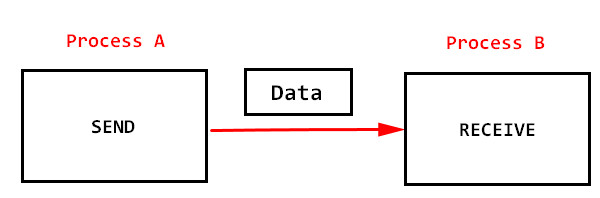
\includegraphics[width=\linewidth]{MPI_design.jpg}
\caption{MPI Design}
\end{figure}
\section{System Organization}

\section{Code Implement}
\subsection*{$Code$}
\lstinputlisting[language=C]{lab.c}
\section{Who did what?}
-  Code implement: Ta Hoang Hai Nam \\
-  MPI design: Ta Hoang Hai Nam \\ 
-  System organization:  Kieu Quoc Viet, Trinh Hoang Hai\\
-  Report: Ta Hoang Hai Nam, Le Sinh Quy.
\end{document}